\documentclass[12pt,letterpaper,noanswers]{exam}
\usepackage[usenames,dvipsnames,svgnames,table]{xcolor}
\usepackage[margin=0.9in]{geometry}
\renewcommand{\familydefault}{\sfdefault}
\usepackage{multicol}
\usepackage{wrapfig}
\pagestyle{head}
\header{AM 22b Class 32}{}{Apr 16: Differential equations, p. \thepage}
\runningheadrule
\headrule
\usepackage{graphicx} % more modern
\usepackage{amsmath} 
\usepackage{amssymb} 
\usepackage{hyperref}
\usepackage{tcolorbox}
\usepackage[utf8]{inputenc}
\usepackage{diagbox}
\usepackage{graphicx} 
\usepackage{enumitem}
\usepackage{tikz}
\tikzstyle{startstop} = [rectangle, rounded corners, minimum width=3cm, minimum height=1cm,text centered, draw=black]

\tikzstyle{process} = [rectangle, minimum width=3cm, minimum height=1cm, text centered, draw=black, fill=gray!20]
\tikzstyle{decision} = [ellipse, minimum width=3cm, minimum height=0.5cm, text centered, draw=black, fill=white!30]
\tikzstyle{arrow} = [thick,->,>=stealth]
\usetikzlibrary{shapes.geometric, arrows}
\pagenumbering{arabic}

\usepackage[numbered,autolinebreaks,useliterate]{mcode}

\newcommand{\mb}[1]{\underline{#1}}

\begin{document}
 \pdfpageheight 11in 
  \pdfpagewidth 8.5in




% I need to review the torus trajectories...

\begin{itemize}
% \item There is a pre-class assignment (20 minutes of videos + a few WeBWorK exercises) due at 10am this Monday.  It is available on Canvas.
\itemsep0em
\item There is a skill check on Monday. (C30, 31, 32)
\item Quiz 05 is available on Gradescope and will be available until Sunday at 6pm ET.
\item PSet 09 will be posted by the end of today, and is due on Thursday April 22nd at 6pm ET.
\end{itemize}

\hrule
\vspace{0.2cm}

% partial derivatives, gradient
% local linearity, differential, directional deriv
% 2nd order partials + equations with partials

\noindent\textbf{Big picture}

We will learn how to analyze differential equations from three perspectives: using approximate solutions (slope fields + Euler's method + RK45), finding exact solutions (rarely, using separation of variables), using qualitative methods (identifying equilibrium solutions and whether they are `stable' or `unstable').

Today we will approximate solutions to differential equations.

\vspace{0.2cm}
\hrule
\vspace{0.2cm}

\noindent\textbf{Skill Check C32 Practice}

\begin{questions}
\item Classify the stability of the equilibrium solutions of $\dfrac{dx}{dt} = x(1-x)(3-x)$.
\end{questions}

\noindent\textbf{Skill Check C32 Practice Solution}

\begin{enumerate}
    \item Find the equilibrium solutions: Equilibrium solutions when $\frac{dx}{dt} = 0$ for some $x$, so $x^* = 0, 1, 3$.
    \item To identify stability, check $f'(x^*)$.
    \item Using the product rule,
$\dfrac{df}{dx} = (1)(1-x)(3-x) + x(-1)(3-x) + x(1-x)(-1)$.
\item Substitute the different equilibrium solutions: 

Substituting $x^* = 0$, $f' = (1)(3) = 3$.  Unstable

Substituting $x^* = 1$, $f' = 1(-1)(2) = -2$.  Stable

Substituting $x^* = 3$, $f' = 3(-2)(-1) = 6$.  Unstable
\end{enumerate}




\emph{Notice that by using the product rule, only one of the three terms was nonzero for each substitution}.


%There will be a Skill Check Retake for Skill Checks C26, C27, C28, C29, C30 on Friday.

\vspace{0.2cm}
\hrule
\vspace{0.2cm}



\noindent\textbf{Teams}
% Dabao, James, Taylor, Akhila, Jonny

\begin{multicols}{2}

1.  student names
\end{multicols}

\vspace{0.2cm}
\hrule
\vspace{0.2cm}


\noindent\textbf{A few properties we've encountered}
\begin{tcolorbox}
\begin{itemize}
\itemsep0em
\item For a linear homogeneous differential equation, the solutions can be added together to generate additional solutions (\textbf{superposition}).  That is not true for nonlinear differential equations or for nonhomogeneous differential equations.
\item A solution to $\dfrac{dx}{dt} = ax$, $a>0$, is either identically $0$ or grows without bound ($x(t) = x(0)e^{at}$).
\end{itemize}
\end{tcolorbox}

\noindent\textbf{Proportional response (linear differential equation)}

For the linear differential equation $\dfrac{dx}{dt} = ax$ the rate of change of the solution, $\frac{dx}{dt}$, is proportional to the state of the system, $x(t)$.

For nonlinear differential equations, the rate of change (the \textbf{response} of the system) cannot be directly proportional to the state.


\noindent\textbf{Time invariance}.  

The solution curves for $\dfrac{dx}{dt} = 0.5x$, $x(0) = 0.2$ and $x(4) = 0.2$ have the same shape.  So do the solution curves for $\dfrac{dx}{dt} = -0.5x$, $x(0) = 3$, $x(4) = 3$.  Why do they have the same shape?

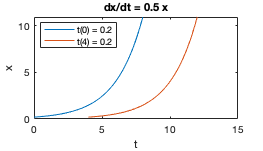
\includegraphics[width=0.45\textwidth]{img/C32p3.png}
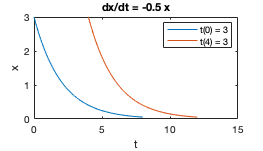
\includegraphics[width=0.45\textwidth]{img/C32p3b.png}



\vspace{1in}



% \noindent\textbf{Exponential growth vs logistic growth}

% \noindent\textbf{Example.  Exponential growth.} Consider the population model $\frac{dP}{dt} = kP$.  Identify the range of $P$ for which $\frac{dP}{dt}$ is positive, negative, or zero.
% \vspace{1in}

% \noindent\textbf{Example.  Logistic growth.} Consider the population model $\frac{dP}{dt} = kP(b - P)$.  Identify the range of $P$ for which $\frac{dP}{dt}$ is positive, negative, or zero.
% \vspace{1in}

% \noindent\textbf{Stability of an equilibrium solution}
% \begin{tcolorbox}
% \begin{itemize}
% \itemsep0em
%     \item 
% \end{itemize}
% \end{tcolorbox}




\vspace{0.2cm}
\hrule
\vspace{0.2cm}


\noindent\textbf{Approximating solutions near an equilibrium: linear approximation}
\begin{tcolorbox}
\begin{itemize}
   
    \item Recall that an \textbf{equilibrium solution} to the differential equation $\frac{dx}{dt} = f(x)$ is a solution of the form $x(t) = x^*$ where $x^*$ is a constant.  For this to be a solution, it must be the case that $f(x^*) = 0$.
\end{itemize}

\end{tcolorbox}
\begin{tcolorbox}
\begin{itemize}
\itemsep0em
 \item We found an exact solution, $x(t) = x_0e^{at}$ to the initial value problem $\dfrac{dx}{dt} = ax$, $x(0) = x_0$.  For other differential equations, given an initial conditions near an equilibrium solution, we will be able to approximate the solution via this linear differential equation.
    \item Consider a differential equation $\dfrac{dx}{dt} = f(x)$.  At equilibrium solutions, $x(t) = x^*$.  For $x(0) - x^*$ small, approximate the differential equation by Taylor expanding.
    \item Taylor expand $f(x)$ about the equilibrium solution to first order.  We find an equation of the form $\frac{dx}{dt} = a(x-x^*)$ where $x^*$ is the equilibrium solution, $x-x^*$ is small, and $a = f'(x^*)$ is a constant. 
    \item Solving the resulting (approximate) differential equation, we find $x(t) \approx x^* + (x(0)-x^*)e^{ct}$ where $c = \left.\frac{df}{dx}\right\vert_{x^*}$.
    \item You can think of a solution $x(t)$ to a nonlinear differential equation $\frac{dx}{dt} = f(x)$ as a combination of exponential growth away from an equilibrium where $f'(x^*)>0$ and exponential decay towards an equilibrium where $f'(x^*)<0$.
\end{itemize}
\end{tcolorbox}
\noindent\textbf{Mathematical details: example}

Let $\dfrac{dx}{dt} = \sin x$.  
\begin{enumerate}
    \item Equilibrium solutions occur at $x^* = k\pi$ for $k\in \mathbb{Z}$ (i.e. for $k$ an integer).
    \item $\dfrac{dx}{dt} \approx f(x^*) + (x-x^*)f'(x^*)$ (Taylor expansion about $x^*$).
    \item This is $\dfrac{dx}{dt}\approx (x-k\pi)\cos(k\pi)$.
    \item $\left\{\begin{array}{l} \dot{x} \approx x - k\pi \text{ for }k\text{ even } \\\dot{x} \approx -(x - k\pi) \text{ for }k\text{ odd } \end{array}
    \right.$
    \item Near $x^*$, 
    $\left\{\begin{array}{l} x(t) \approx k\pi + (x-k\pi)e^t \text{ for }k\text{ even } \\ x(t) \approx k\pi + (x-k\pi)e^{-t} \text{ for }k\text{ odd } \end{array}
    \right.$
\end{enumerate}

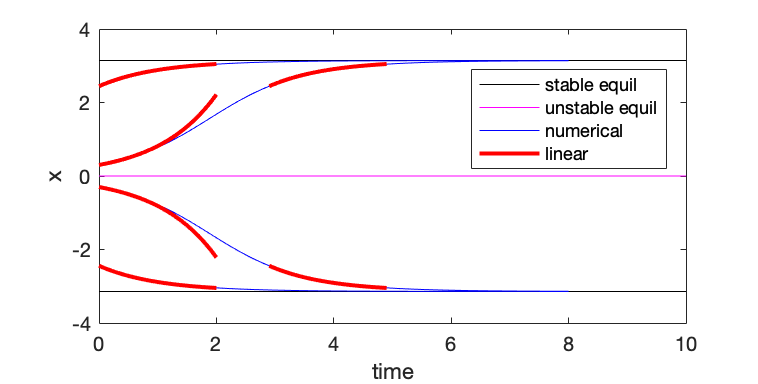
\includegraphics[scale=0.3]{img/C31p1.png}

    \vspace{0.2cm}
\hrule
\vspace{0.2cm}

\noindent\textbf{Stability of an equilibrium solution}
\begin{tcolorbox}
We call an equilibrium solution \textbf{stable} if nearby solutions decay towards it ($f'(x^*)<0$: nearby solutions are approximated by a decaying exponential).  We call it \textbf{unstable} if nearby solutions grow away from it ($f'(x^*)>0$: nearby solutions are approximated by a growing exponential).  \emph{We leave the $f'(x^*) = 0$ case alone for now}.
\end{tcolorbox}


     \noindent\textbf{Example}
     \begin{enumerate}
     \item Classify the equilibrium solutions of $\dfrac{dx}{dt} = ax - bx^2$, with $a,b>0$ as stable or unstable.
     \vspace{1.5in}
     
     \item Use linear approximation to write down an approximate solution for $\dfrac{dx}{dt} = ax - bx^2$, $x(0) = x^* + 0.3$ where $x^*$ is the larger of your equilibrium solutions.
     \vspace{1.5in}
     
     \item Classify the stability of the equilibrium solutions of $\dfrac{dx}{dt} = x(1-x)(3-x)$.
     
     \end{enumerate}
     
    
    \vspace{0.2cm}
\hrule
\vspace{0.2cm}


% \noindent\textbf{Dimension}
% \begin{tcolorbox}
% \begin{itemize}
% \itemsep0em
%     \item Consider $\dfrac{dx}{dt} = ax$.  $\left[\dfrac{dx}{dt}\right] = \dfrac{[x]}{[t]}$ so $[ax] = [x]/[t] \Rightarrow [a] = \dfrac{1}{[t]}$.  $a$ is referred to as a rate.  It has dimensions of inverse time.  $1/a$ has dimensions of time, and sets a timescale of growth or decay of solutions.
%     \item Through a process called \textbf{non-dimensionalizing}, it is possible to substitute a variable or constant that has dimensions of $1$ for a variable or constant with another dimension.
% \end{itemize}
% \end{tcolorbox}

% \noindent\textbf{Rescale time to eliminate a parameter}

% Consider $\dfrac{dx}{dt} = ax, x(0) = x_0$, with solution curve $x(t) = x_0 e^{at}$.  Let $t_{new} = at$.
% \begin{enumerate}
%     \item Rewrite the solution curve in the new time variable, as $x(t_{new}$.
%     \vspace{0.7in}
    
%     \item Use the chain rule to write a differential equation in the new variable, so with $\dfrac{dx}{dt_{new}}$ as the derivative in the equation.
%     \vspace{1.5in}
    
% \end{enumerate}

% 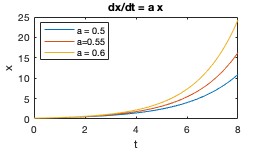
\includegraphics[width=0.45\textwidth]{img/C32p4a.png}
% 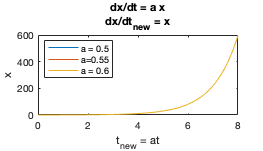
\includegraphics[width=0.45\textwidth]{img/C32p4b.png}


%     \vspace{0.2cm}
% \hrule
% \vspace{0.2cm}

% \noindent\textbf{Approximating solutions: error in numerical methods}
% \begin{tcolorbox}
% \begin{itemize}
%   \item For the initial value problem $\dfrac{dx}{dt} = f(x)$, $x(0) = x_0$, we have seen the \textbf{forward Euler method} of approximating a solution: with this method, we approximation the solution curve $x(t)$ with $x(0) = x_0$ by a series of points of the form $(t_k, x_k)$ where $t_k = k\Delta t$, $x_1 = x_0 + \Delta t f(x_0)$ and $x_{n+1} = x_n + \Delta t f(x_n)$.
%   \item We can think about this method via a Taylor expansion:  assume $x_n$ is an approximation to $x(t)$ after $n$ time steps (at time $t_n$) and $h = \Delta t$ is a small time step.  Approximate $x_{n+1}$ at time $t_{n+1} = t_n + h$, given the approximation $x_n$ at time $t_n$.  $x_{n+1} \approx x(t_n+h)$ where $h$ is a small amount of time.  Taylor expanding, $x_{n+1}\approx x(t_n+h) \approx x(t_n) + h \left.\frac{dx}{dt}\right\vert_{x(t_n)} \approx x_n + h f(x_n)$.  
%   \item The first term of the Taylor expansion that is dropped is the $h^2$ term, so we say that this method has an error of order $h^2$ in calculating $x_{n+1}$ based on $x_n$.  However, $x_n$ was itself an approximation of $x(t_n)$, and over successive steps the error builds.  It turns out the overall error of this method is order $h$.  We call the method a \textbf{first order method}.


  
%     \item In Euler's method, the slope $f(x_n)$ at a single point, $(t_n, x_n)$, is used to approximate the slope of $x(t)$ over the entire time interval from $t_n$ to $t_{n+1}$
%     \end{itemize}
%     \end{tcolorbox}
%     \begin{tcolorbox}
%     \begin{itemize}
%     \itemsep0em
%     \item In practice, other methods of approximating are more often used.  The \textbf{Runge-Kutta 4} method involves combining four different approximations of $\dfrac{dx}{dt}$ on the interval $t_n\leq t\leq t_{n+1}$ to produce $x_{n+1}$ from $x_n$.  In RK4, $x_{n+1} = x_n + h\left(\frac{k_1}{6}+\frac{2k_2}{6}+\frac{2k_3}{6}+\frac{k_4}{6}\right)$, where $k_1, k_2, k_3, k_4$ are each a different approximation of $f(x(t))$ on the time interval $t_n\leq t\leq t_{n+1}$.  
%     \item For RK4, the local error over a single step is order $h^5$ while the overall error over many steps is order $h^4$ so the method is referred to as \textbf{fourth order}.
% \end{itemize}
% \end{tcolorbox}

% \noindent\textbf{Example}

% Compare RK4 with forward Euler for $\dfrac{dx}{dt} = 0.8x$.

% 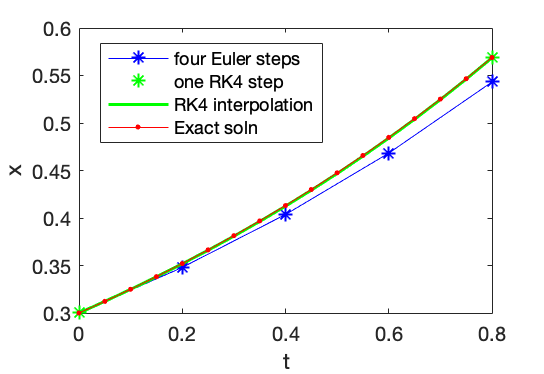
\includegraphics[scale=0.5]{img/C32p2.png}

% \begin{enumerate}
%     \item Why might it make sense to compare one step of RK4 to four steps of forward Euler?
    
% \vfill
    
%     \item The RK4 interpolation is a polynomial in $t$.  It passes through $x_0$ at $t_0$, through $x_1$ at $t_1$, and has a slope given by $k_1$ at $(t_0,x_0)$ and by $k_4$ at $(t_1,x_1)$.  How many terms are needed in the polynomial to be able to meet these conditions?
% \end{enumerate}

% \vfill




\end{document}